\documentclass[tikz,border=3pt]{standalone}
\usepackage[utf8]{inputenc}
\usepackage[T1]{fontenc}
\usepackage{lmodern}
\renewcommand{\familydefault}{\sfdefault}
\usepackage{sansmath}\sansmath
\usepackage{chemfig}
\usepackage{pgfplots}\pgfplotsset{compat=1.18,/pgf/number format/use comma,/pgf/number format/1000 sep={.}}
\usetikzlibrary{arrows.meta,calc,positioning,decorations.pathmorphing,patterns}
% paleta del sitio
\definecolor{nar}{HTML}{E8680C}\definecolor{narc}{HTML}{FFB35C}\definecolor{hielo}{HTML}{FFF3E8}
\definecolor{tinta}{HTML}{1D1D1F}\definecolor{gris}{HTML}{6E6E73}\definecolor{lila}{HTML}{7C5CF0}
\definecolor{azul}{HTML}{2F6FD6}\definecolor{menta}{HTML}{17A673}\definecolor{coral}{HTML}{E8342A}
\begin{document}
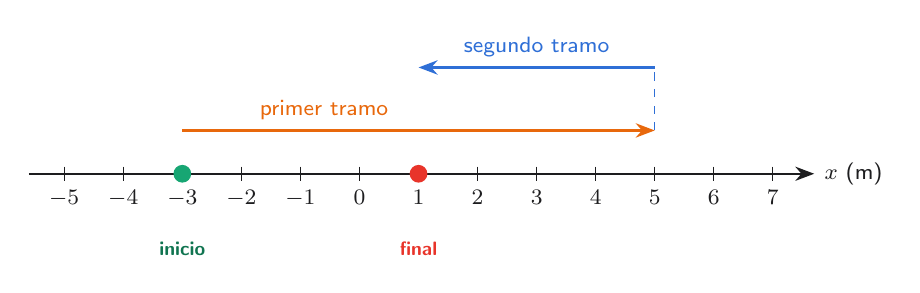
\begin{tikzpicture}[font=\footnotesize,>={Stealth[length=2.4mm]},x=0.75cm]
\draw[->,thick,tinta] (-5.6,0) -- (7.7,0) node[right] {$x$ (m)};
\draw[tinta] (-5,0.09) -- (-5,-0.09) node[below] {$-5$};
\draw[tinta] (-4,0.09) -- (-4,-0.09) node[below] {$-4$};
\draw[tinta] (-3,0.09) -- (-3,-0.09) node[below] {$-3$};
\draw[tinta] (-2,0.09) -- (-2,-0.09) node[below] {$-2$};
\draw[tinta] (-1,0.09) -- (-1,-0.09) node[below] {$-1$};
\draw[tinta] (0,0.09) -- (0,-0.09) node[below] {$0$};
\draw[tinta] (1,0.09) -- (1,-0.09) node[below] {$1$};
\draw[tinta] (2,0.09) -- (2,-0.09) node[below] {$2$};
\draw[tinta] (3,0.09) -- (3,-0.09) node[below] {$3$};
\draw[tinta] (4,0.09) -- (4,-0.09) node[below] {$4$};
\draw[tinta] (5,0.09) -- (5,-0.09) node[below] {$5$};
\draw[tinta] (6,0.09) -- (6,-0.09) node[below] {$6$};
\draw[tinta] (7,0.09) -- (7,-0.09) node[below] {$7$};
\fill[menta] (-3,0) circle (3.2pt);
\fill[coral] (1,0) circle (3.2pt);
\node[text=menta!70!black,font=\scriptsize\bfseries] at (-3,-0.95) {inicio};
\node[text=coral,font=\scriptsize\bfseries] at (1,-0.95) {final};
\draw[->,very thick,nar] (-3,0.55) -- (5,0.55) node[pos=0.3,above] {primer tramo};
\draw[azul,dashed] (5,0.55) -- (5,1.35);
\draw[->,very thick,azul] (5,1.35) -- (1,1.35) node[midway,above] {segundo tramo};
\end{tikzpicture}
\end{document}
